% fig3_estimator_agreement.tex
%
% Two estimators, one answer. The per-cell DINN reaches `scav_rat` by backpropagation and
% returns a point estimate per cell; EKI reaches it with no gradients at all and returns a
% spread. Both land below Carroll. Because they share no optimiser, the agreement is
% evidence about the data rather than about either method.
%
% ---------------------------------------------------------------------------------------
% STRUCTURE AND STYLING ADAPTED FROM tikz.net, WITH THANKS:
%   "Regular vs Bayes NN"  https://tikz.net/regular-vs-bayes-nn/
%       the \nn{<suffix>} macro that draws one network twice under different node names,
%       the two-argument `edge` style whose pos is staggered by (mod(#1+#2,2)+1)*0.33 so
%       edge labels never collide, and the `distro` style that draws a Gaussian inside a
%       node via `path picture` instead of a hand-shifted scope.
%   "Neural networks"      https://tikz.net/neural_networks/
%       the palette method: every hue is mixed toward black (red!80!black), and one base
%       hue yields a text / draw / fill triple at different mixes.
% The construction is theirs. The content, the labels and the result are ours.
% ---------------------------------------------------------------------------------------
%
%   pdflatex fig3_estimator_agreement.tex
%
\documentclass[tikz,border=8pt]{standalone}
\usetikzlibrary{calc,arrows.meta,positioning}

% ---- palette: mixed toward black, never a raw hue ------------------------------------
\colorlet{myblue}{blue!80!black}
\colorlet{myred}{red!80!black}
\colorlet{mygreen}{green!60!black}
\colorlet{myorange}{orange!85!black}
\colorlet{mydarkblue}{blue!40!black}
\colorlet{myink}{black!80}

\def\layersep{2.6cm}

% One network, drawn twice under different node suffixes.
\newcommand\nn[1]{
  % inputs: what the network sees
  \foreach \y [count=\i] in {2.35, 1.15}
    \node[node in] (i\i-#1) at (0,\y) {};
  % trunk
  \foreach \y [count=\i] in {3.0, 2.0, 1.0, 0.0}
    \node[node hidden] (h\i-#1) at (\layersep,\y) {};
  % the parameter that is actually in dispute
  \node[node out] (o-#1) at (2*\layersep,1.5) {};

  \foreach \source in {1,...,2}
    \foreach \dest in {1,...,4}
      \path (i\source-#1) edge (h\dest-#1);
  \foreach \source in {1,...,4}
    \path (h\source-#1) edge (o-#1);
}

\begin{document}
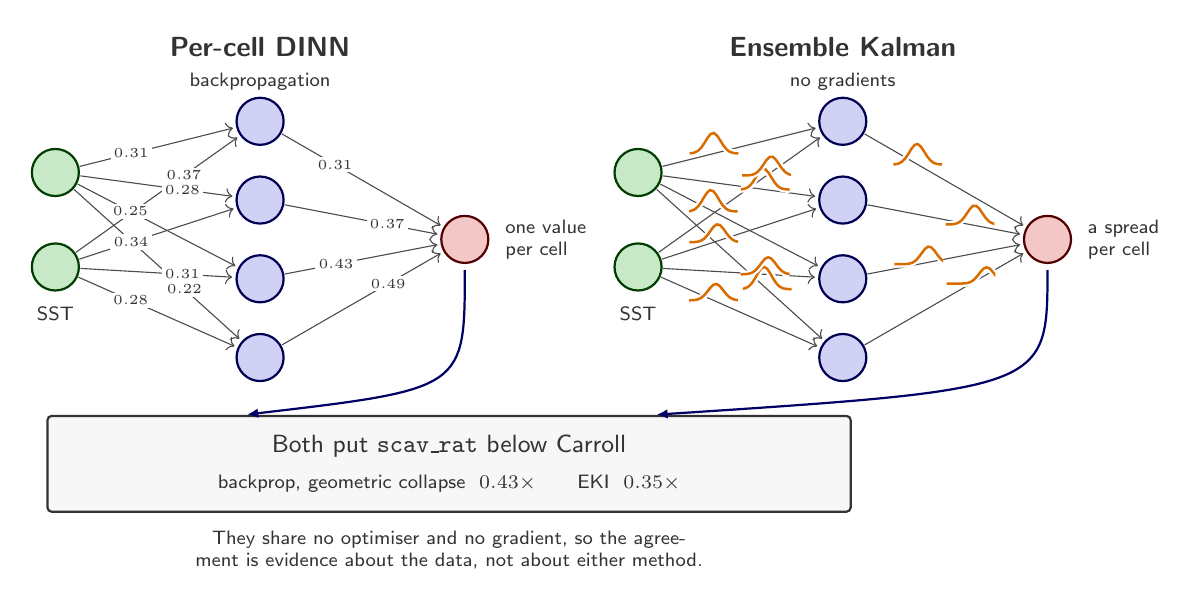
\begin{tikzpicture}[
    shorten >=1pt, ->, draw=black!70, node distance=\layersep,
    font=\sffamily,
    node/.style={thick, circle, draw=myblue, minimum size=17, inner sep=0.5, outer sep=0.6},
    node in/.style    ={node, mygreen!20!black, draw=mygreen!40!black, fill=mygreen!22},
    node hidden/.style={node, myblue!20!black,  draw=myblue!40!black,  fill=myblue!18},
    node out/.style   ={node, myred!20!black,   draw=myred!40!black,   fill=myred!22},
    % stagger label positions along the edge so neighbours never overlap
    edge/.style 2 args={pos={(mod(#1+#2,2)+1)*0.33}, font=\tiny},
    weight/.style 2 args={
      edge={#1}{#2}, fill=white, inner sep=1.2pt, text=myink,
      node contents={\pgfmathparse{0.28+0.06*#1-0.03*#2}\pgfmathprintnumber[fixed,precision=2]{\pgfmathresult}}
    },
    % a spread rides the edge instead of a scalar; mean and width vary per edge
    distro/.style 2 args={
      edge={#1}{#2}, node contents={}, minimum size=0.62cm,
      % mean shifts with #1 and width with #2, so no two edges carry the same posterior.
      % The skew is kept low: past about 1.2 the curve stops reading as a distribution.
      path picture={\draw[double=myorange, white, thick, double distance=0.9pt, shorten >=0pt]
        plot[variable=\t, domain=-1:1, samples=51]
        ({\t},{0.26*exp(-55*(\t-0.07*(#1-1))^2 - 1.1*\t*#2)});}
    },
    caption/.style={font=\sffamily\small, text=myink},
    banner/.style={draw=myink, thick, rounded corners=1.5pt, fill=black!3,
                   align=center, inner sep=7pt, font=\sffamily\small, text=myink},
  ]

  % ------------------------------------------------------------------ left: backprop
  \nn{grad}
  \node[caption, font=\sffamily\bfseries] at (\layersep,3.95) {Per-cell DINN};
  \node[caption, font=\sffamily\scriptsize] at (\layersep,3.5) {backpropagation};

  % ------------------------------------------------------------------ right: EKI
  \begin{scope}[xshift=7.4cm]
    \nn{eki}
    \node[caption, font=\sffamily\bfseries] at (\layersep,3.95) {Ensemble Kalman};
    \node[caption, font=\sffamily\scriptsize] at (\layersep,3.5) {no gradients};
  \end{scope}

  % point estimates on every gradient-side edge
  \foreach \i in {1,...,2}
    \foreach \j in {1,...,4}
      \path (i\i-grad) -- (h\j-grad) node[weight={\i}{\j}];
  \foreach \i in {1,...,4}
    \path (h\i-grad) -- (o-grad) node[weight={\i}{1}];

  % distributions on every ensemble-side edge
  \foreach \i in {1,...,2}
    \foreach \j in {1,...,4}
      \path (i\i-eki) -- (h\j-eki) node[distro={\i}{\j}];
  \foreach \i in {1,...,4}
    \path (h\i-eki) -- (o-eki) node[distro={\i}{1}];

  % ------------------------------------------------------------------ labels + result
  \node[caption, font=\sffamily\scriptsize, below=2pt of i2-grad]  {SST};
  \node[caption, font=\sffamily\scriptsize, below=2pt of i2-eki]   {SST};
  \node[caption, font=\sffamily\scriptsize, right=2pt of o-grad, align=left]
        {one value\\per cell};
  \node[caption, font=\sffamily\scriptsize, right=2pt of o-eki, align=left]
        {a spread\\per cell};

  \node[banner, minimum width=10.2cm] (agree) at (5.0,-1.35)
    {Both put {\ttfamily scav\_rat} below Carroll\\[2pt]
     {\scriptsize backprop, geometric collapse\ \ $0.43\times$\qquad EKI\ \ $0.35\times$}};

  \draw[-{Latex[length=4,width=3.5]}, thick, mydarkblue, shorten <=2pt]
        (o-grad) .. controls (2*\layersep,-0.4) .. ([xshift=-2.6cm]agree.north);
  \draw[-{Latex[length=4,width=3.5]}, thick, mydarkblue, shorten <=2pt]
        (o-eki)  .. controls (7.4cm+2*\layersep,-0.4) .. ([xshift=2.6cm]agree.north);

  \node[caption, font=\sffamily\scriptsize, below=3pt of agree, text width=10.2cm,
        align=center]
    {They share no optimiser and no gradient, so the agreement is evidence about the data,
     not about either method.};

\end{tikzpicture}
\end{document}
